\subsection{Post-hoc Coordinates after Nonlinear Learning}\label{app:posthoc_chart}

The frozen-trunk control removes reference inference but also restricts learning.
Here both nonlinear layers remain trainable throughout continuation. Only after
training do we fit an affine chart from new features into the old coordinates.
This tests the utility and compatibility attainable through established linear
alignment, rather than introducing a new alignment family.

With row-vector features, write the current logits as $hW^\top+\beta$.
An invertible chart emits $\widetilde h=hM+b$. Rebasing the current head by
\begin{equation}
 W'{}^\top=M^{-1}W^\top,\qquad
 \beta'=\beta-bM^{-1}W^\top
 \label{eq:chart_rebase}
\end{equation}
preserves these logits in real arithmetic. Composing the chart with the
encoder's final affine layer leaves its shapes unchanged. This elementary
reparameterization preserves the current head; recovery of the old consumer
depends on how well the fitted chart describes its drift.

The committed protocol uses three development seeds $600$--$602$ per task.
HAR reconstructs inputs with $10\%$ of fitting primary labels, dose $10$ and
$60+30$ epochs; RadioML predicts SNR with $20\%$, dose $1$ and $25+25$ epochs.
Both use width $64$, Adam $10^{-3}$, batch $256$, fp32 nonlinear layers and a
float64 final affine map. D/J clone the healthy model and complete optimizer
state and share future minibatches. All nonlinear trunks change. Development
evaluates validation only. Each chart uses $1{,}024$ uniformly sampled fitting
inputs, with no labels. Old anchor features are cached offline.

Two fixed candidates are checked in order: diagonal statistics, then paired
ridge with standardized coefficient $10^{-3}$. Singular values of the raw
coordinate map are floored at $10^{-3}$ of the largest before rebasing.
The development gate requires positive mean J--D, old accuracy within $0.5$
point of healthy, NLL increase at most $0.05$, ECE increase at most $0.02$,
unchanged current predictions with logit error below $10^{-8}$, identical
encoder shapes, and mean latency ratios at most $1.20/1.10$ for batches
$1/1{,}024$. HAR fails the auxiliary-benefit gate. SNR diagonal repair fails
ECE; paired ridge passes and alone opens confirmation.

\begin{table}[t]
\centering
\caption{Post-hoc single-encoder chart, ten independent SNR confirmation seeds. Means on the full fixed test corpus. Current logits are algebraically preserved by head rebasing. Old-reader metrics can improve despite extensive prediction changes. The five-point disagreement budget certifies none of the ten repaired joint consumers.}
\label{tab:chart_confirmation}
\footnotesize
\begin{tabular}{lrrrr}
\toprule
Consumer & accuracy & NLL & ECE & changed predictions \\
\midrule
Healthy old & 0.251 & 2.044 & 0.043 & 0 \\
Native J, old readout & 0.260 & 2.168 & 0.166 & 56.69\% \\
Chart J, old readout & 0.264 & 1.984 & 0.019 & 44.07\% \\
Native J, current head & 0.281 & 1.980 & 0.053 & --- \\
Chart J, rebased current & 0.281 & 1.980 & 0.053 & 0 (vs. native J) \\
Supervised refit & 0.285 & 1.993 & 0.070 & --- \\
\bottomrule
\end{tabular}
\end{table}


Ten fixed new seeds $700$--$709$ receive the unchanged SNR recipe. A user-requested
inventory interrupted the queue; complete records were retained and only the
missing final seed was rerun, with the stop and resume provenance preserved.
Current J--D is $\ChartGain$ points, paired descriptive $95\%$ interval
$[\ChartGainLow,\ChartGainHigh]$. Rebasing preserves every current prediction;
maximum logit error is $1.44\times10^{-12}$. The old consumer improves from
$\ChartHealthy$ healthy accuracy to $\ChartRepairedOld$, a difference of
$\ChartOldGain$ points, $[\ChartOldGainLow,\ChartOldGainHigh]$. Mean NLL and ECE
decrease by $0.0604$ and $0.0242$. Native J reaches $\ChartCurrent$ current
accuracy; the supervised refit reaches $0.285$. These are low-label measurements
on the fixed prepared modulation split, not competitive benchmark claims.

\begin{figure}[t]
\centering
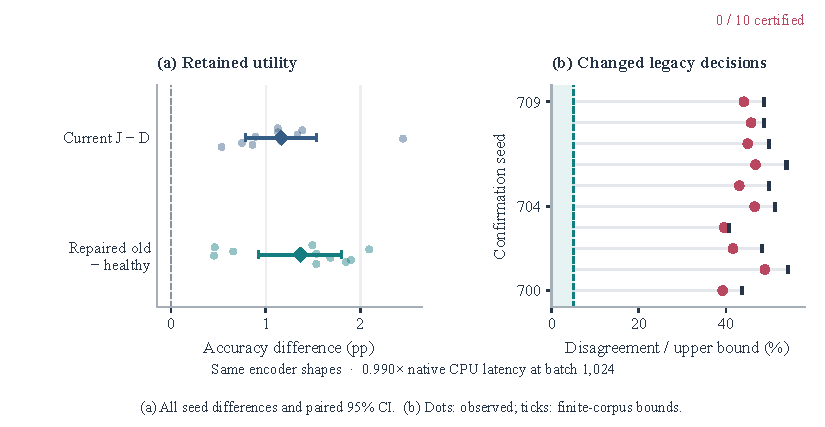
\includegraphics[width=\linewidth]{figures/fig_chart_confirmation.pdf}
\caption{A folded chart retains utility at native encoder cost but changes many
legacy decisions. (a) All ten seed differences and paired $95\%$ intervals.
(b) Repaired-J disagreement with healthy predictions and simultaneous
finite-corpus upper bounds. Every bound exceeds the five-point budget.
Healthy aggregate accuracy is $\ChartHealthy$; a higher aggregate score does
not imply decision compatibility.}
\label{fig:chart_confirmation}
\end{figure}

The complete target fails. The repaired consumers change $\ChartDisagreement\%$
of healthy predictions on average. A separate forty-consumer family uses total
$\delta=0.05$, $1{,}024$ uniform monitor inputs and a $0.05$ error budget.
None of the ten repaired joint consumers certifies; their upper remainder
disagreement bounds range from $0.406$ to $0.543$. This is abstention by the
declared check, not evidence that classification error increased: the paired
accuracy differences are positive. The result distinguishes an accuracy repair
from preserving old decisions.

On one CPU thread, alternating $31$ timed repetitions after five warm-ups give
mean median-latency ratios $0.900$ at batch $1$ and $\ChartLatency$ at batch
$1{,}024$. Both branches evaluate final-affine features and primary logits in
float64. The rebased head stores float64 parameters; the native fp32 head is
cast for logit evaluation. We interpret the result as near-native encoder cost,
not an algorithmic speedup. Auxiliary heads are not included in these primary
inference timings. The chart and current heads are composed offline; inference
does not require the reference encoder or a separate projection. Fitting still
requires anchor feature extraction and matrix estimation, not constant time.

All native model/Adam states, fitted charts, deployed models, source hashes and
timing samples are retained locally. Drivers are \texttt{posthoc\_chart\_cpu.py}
and its frozen confirmation wrapper; analysis is
\texttt{summarize\_posthoc\_chart.py}. The original grid is not extended after
the failed conjunction.
